\documentclass[twoside]{article}
\usepackage{aistats2016}
\usepackage{graphicx}
\graphicspath{{picF/}}
\usepackage{amsmath,amssymb,amsbsy,amsfonts,amsthm}
\usepackage{tikz}
\usetikzlibrary{arrows,decorations.pathmorphing,backgrounds,positioning,fit}

\newcommand{\vvmK}{\dot{\eta}}
\newcommand{\vvmW}{\dot{\zeta}}
\newcommand{\vvmDK}{\dot{\alpha}}
\newcommand{\vvmKW}{\dot{\beta}}
\newcommand{\vvmbDK}{\bar{\alpha}}
\newcommand{\vvmbKW}{\bar{\beta}}
\newcommand{\vvmDWK}{\mu}
\newcommand{\pmK}{\eta}
\newcommand{\pmW}{\zeta}
\newcommand{\vmK}{\alpha}
\newcommand{\vmW}{\beta}
\newcommand{\vmDK}{\theta}
\newcommand{\vmKW}{\phi}

\newcommand{\pr}{\mathbf{p}}
\newcommand{\dd}{\mathbf{d}}
\newcommand{\divergence}{\mathbb{K}}
\newcommand{\entropy}{\mathbb{H}}
\newcommand{\expectation}{\mathbb{E}}
\newcommand{\carac}[1]{\mathbb{I}[{#1}]}
\newcommand{\mbeta}{\mathbf{Boojum}}
\newcommand{\cpnt}[2]{{#1}^{(\!{#2}\!)}}
\newcommand{\assignn}{\leftarrow}
\newcommand{\assign}[1]{\underset{\textbf{[#1]}}{\leftarrow}}
\newcommand{\ruleref}[1]{\textbf{[#1]}}

\newtheorem{definition}{Definition}
\newtheorem{lemma}{Lemma}
\newtheorem{proposition}{Proposition}

\tikzset{BNVar/.style={circle,draw}}
\tikzset{BNVarDiscrete/.style={rectangle,draw}}
\tikzset{BNObserved/.style={fill=black!15}}


% If your paper is accepted, change the options for the package
% aistats2016 as follows:
%
%\usepackage[accepted]{aistats2016}

\begin{document}

% If your paper is accepted and the title of your paper is very long,
% the style will print as headings an error message. Use the following
% command to supply a shorter title of your paper so that it can be
% used as headings.
%
%\runningtitle{I use this title instead because the last one was very long}

% If your paper is accepted and the number of authors is large, the
% style will print as headings an error message. Use the following
% command to supply a shorter version of the authors names so that
% they can be used as headings (for example, use only the surnames)
%
%\runningauthor{Surname 1, Surname 2, Surname 3, ...., Surname n}

\twocolumn[

\aistatstitle{On Latent Dirichlet Allocation Priors and Variational Bayes}

\aistatsauthor{ Jean-Marc Andreoli \And Adrien Dulac \And Eric Gaussier }

\aistatsaddress{ Xerox Research Centre Europe\\ Grenoble, France \And Universit{\'e} Grenoble Alpes\\ Laboratoire d'Informatique de Grenoble \And } ]

\begin{abstract}
Latent Dirichlet Allocation (LDA) is a successful model capable of explaining large document collections using a small number of topics. Several methods exist to estimate it, one of the earliest one being Variational Bayes. While the core of the model has been stable since its inception ca. 2003, its ``border'', namely the treatment of the hyper-parameters, has been widely debated, since its importance in practice has been acknowledged. We propose here a new variant of LDA, concerning the choice of its prior, simply applying the principle of Bayesian conjugacy which underlies the rest of its design. This leads to new, efficient update rules for the variational Bayes estimation algorithm, which we discuss and experiment on a few document collections.
\end{abstract}

\section{INTRODUCTION}
One of the earliest applications of the Variational Bayes method in machine learning was in the domain of topic modelling, with the LDA model, where potentially large document collections are summarised by a small set of topics, each document being seen as a sparse mixture of topics and each topic as a sparse mixture of words. Part of the success of the method originates in the simplicity of its algorithm, which relies on a small set of well founded update rules. While the rules associated to the core of the LDA model are stable and consensual, those dealing with the ``border'' of the model have often been debated, and no clear consensus has emerged. In the Bayesian network terminology, the problem is that of the choice of priors, the importance of which has often been acknowledged. We propose here a systematic study of this problem, as well as yet another variant of LDA obtained by simple application of its underlying design principle, which can be informally summarised as: in the absence of better criterion, try conjugate priors.
\section{RELATED WORK}

The LDA model \cite{blei_latent_2003} has been extended in many different ways to address different problems. Information about document authorship has, for example, been added to the model in \cite{Rosen_Zvi_2004}, whereas the integration of correlations between topics in the model has been explored in \cite{blei_correlated_2007}; more recently, \cite{Boyd_Graber_2009} describes an extension to model multilingual unaligned collections. Other extensions have focused on streaming or online versions of the model: \cite{Yao_2009} focuses on efficient methods for inference in streaming collections, whereas \cite{Wang_2012} introduces a new model for text streams based on transition probabilities between topics of successive documents and \cite{hoffman_online_2010} proposes an online variational Bayes algorithm for LDA based on mini-batches.




\section{A CONJUGATE PRIOR FOR THE DIRICHLET DISTRIBUTION}
\label{sec:huntingsnark}
It is well known that the exponential family of distributions satisfies important stability properties, which lead to elegant, analytical expressions in Bayesian inference, hence its massive use in Bayesian models. One property is that any distribution in that family has a natural conjugate also in that family, and there is a systematic procedure to compute it. For example, the Dirichlet distribution can be derived in this way as a conjugate to the multinomial distribution, and they are both in the exponential family. In the sequel, we are interested in a conjugate to the Dirichlet itself, which is easy to derive by application of the same systematic procedure. We name it here the $\mbeta$ distribution\footnote{a.k.a. the Snark distribution, because the Snark is a Boojum, you see.}, for lack of a better name. It is a distribution over the positive orthant $\mathbb{R}_+^N$ (the parameter space of the $N$-dimensional Dirichlet), and has two parameters $m,\boldsymbol{\tau}$ where $m\in\mathbb{R}$ is a scalar and $\boldsymbol{\tau}\in\mathbb{R}^N$ is a vector (as a general rule, the parameter space of the conjugate has dimension one plus the dimension of the parameter space of the original distribution). It is defined, for $\boldsymbol{x}\in\mathbb{R}_+^N$ by
\begin{eqnarray}
\mbeta(\boldsymbol{x};m,\boldsymbol{\tau}) & \triangleq & \frac{1}{Z(m,\boldsymbol{\tau})}\mathcal{B}(\boldsymbol{x})^m\exp-\boldsymbol{\tau}\boldsymbol{x}
\end{eqnarray}
where $\mathcal{B}$ denotes the multivariate beta function $\mathcal{B}(\boldsymbol{x})\triangleq\frac{\prod_n\Gamma(x_n)}{\Gamma(\sum_nx_n)}$ which is also the normalising constant of the Dirichlet distribution with parameter $\boldsymbol{x}$, and $Z(m,\boldsymbol{\tau})$ is the normalising constant of the $\mbeta$ distribution itself, defined by
\begin{eqnarray*}
Z(m,\boldsymbol{\tau}) & \triangleq & \int_{\boldsymbol{x}\in\mathbb{R}_+^N}\mathcal{B}(\boldsymbol{x})^m\exp-\boldsymbol{\tau} \boldsymbol{x}\;\dd{\boldsymbol{x}}
\end{eqnarray*}
The expression $\boldsymbol{\tau} \boldsymbol{x}$ in the definition denotes the scalar product of the two vectors. Of course, for the distribution to be proper, the normalising constant must be finite, which is not always the case. Although no analytical formula is known for $Z(m,\boldsymbol{\tau})$, one exists for its finiteness:
\begin{proposition}
\label{prop:mbeta-proper}
The distribution $\mbeta(m,\boldsymbol{\tau})$ is proper, i.e. $Z(m,\boldsymbol{\tau})<\infty$, if and only if\footnote{For any whole number $N$, we use the shorthand $n\in N$ to mean $n\in\{1\ldots N\}$}
\[
\begin{array}{l}
\forall n\in N\;\tau_n>0 \;\textrm{ and }\; m<1 \;\textrm{ and }\\
(m\geq0 \;\textrm{ or }\; \sum_{n\in N}\exp-\frac{\tau_n}{|m|}<1)
\end{array}
\]
\end{proposition}
Now, conjugacy with the Dirichlet distribution is expressed by the following property.
\begin{proposition}
Let $(\boldsymbol{y}_p)_{p\in P}$ be a family of random variables over the simplex of $\mathbb{R}_+^N$, which are mutually independent given a random variable $\boldsymbol{x}$ over $\mathbb{R}_+^N$. We have
\[
\begin{array}{l}
\begin{array}{ll}
\textrm{Prior:} & \boldsymbol{x} \sim \mbeta(m,\boldsymbol{\tau})\\
\textrm{Observation:} & \forall p\in P\;\boldsymbol{y}_p|\boldsymbol{x} \sim \mathbf{Dirichlet}(\boldsymbol{x})\\
\Longrightarrow
\textrm{Posterior:} &
\boldsymbol{x}|(\boldsymbol{y}_p)_{p\in P} \sim \mbeta(m',\boldsymbol{\tau}')
\end{array}\\
\textrm{where } m'=m-|P|\;\;\boldsymbol{\tau}'=\boldsymbol{\tau}-\sum_{p\in P}\log\boldsymbol{y}_p
\end{array}
\]
This holds whenever the prior is proper, in which case so is the posterior.
\end{proposition}
%%%%%%%%%%%%%%%%%%%%%%%%%%%%%%%%%%%%%%%%%%%%%%%%%%%%%%%%%%%%%%%%%%%%%%%%%%%
\section{The LDA model revisited}
%%%%%%%%%%%%%%%%%%%%%%%%%%%%%%%%%%%%%%%%%%%%%%%%%%%%%%%%%%%%%%%%%%%%%%%%%%%
\begin{figure*}
\begin{tabular}{c@{\hspace{1cm}}c}
\begin{minipage}{6cm}
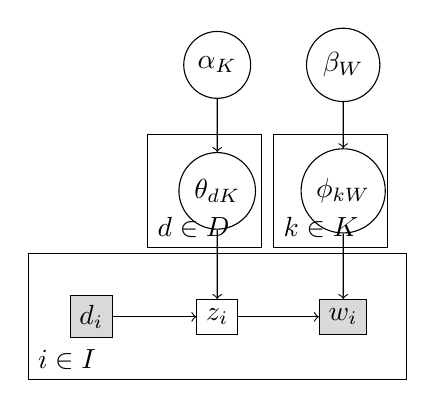
\begin{tikzpicture}[scale=.8]
\node (d) at (0,0) [BNVarDiscrete,BNObserved] {$d_i$};
\node (z) at (2,0) [BNVarDiscrete] {$z_i$};
\node (w) at (4,0) [BNVarDiscrete,BNObserved] {$w_i$};
\node (theta) at (2,2) [BNVar] {$\vmDK_{dK}$};
\node (phi) at (4,2) [BNVar] {$\vmKW_{kW}$};
\node (alpha) at (2,4) [BNVar] {$\vmK_K$};
\node (beta) at (4,4) [BNVar] {$\vmW_W$};
\draw [->] (d) -- (z);
\draw [->] (z) -- (w);
\draw [->] (alpha) -- (theta);
\draw [->] (theta) -- (z);
\draw [->] (beta) -- (phi);
\draw [->] (phi) -- (w);
\draw (-1,-1) rectangle (5,1);
\draw (-1,-1) node[above right] {$i\in I$};
\draw (.9,1.1) rectangle (2.7,2.9);
\draw (.9,1.1) node[above right] {$d\in D$};
\draw (2.9,1.1) rectangle (4.7,2.9);
\draw (2.9,1.1) node[above right] {$k\in K$};
\end{tikzpicture}
\end{minipage} &
$
\begin{array}{l}
\begin{array}{l}
p(\vmK_K\vmW_W\vmDK_{DK}\vmKW_{KW}z_Iw_I|d_I) =\\
\hspace{1cm}p(\vmK_K)p(\vmW_W)\\
\hspace{1cm}\prod_{d\in D}p(\vmDK_{dK}|\vmK_K)\prod_{k\in K}p(\vmDK_{kW}|\vmW_W)\\
\hspace{1cm}\prod_{i\in I}p(z_i|d_i\vmDK_{DK})p(w_i|z_i\vmKW_{KW})
\end{array}
\vspace{.3cm}
\\
\begin{array}{rcl@{\hspace{.5cm}}rcl}
\vmK_K & \sim & \cpnt{p}{K} & \vmW_W & \sim & \cpnt{p}{W}
\end{array}
\\
\begin{array}{r@{\hspace{.5cm}}rcl}
\forall d\in D & \vmDK_{dK}|\vmK_K & \sim & \mathbf{Dirichlet}(\vmK_K)\\
\forall k\in K & \vmKW_{kW}|\vmW_W & \sim & \mathbf{Dirichlet}(\vmW_W)\\
\forall i\in I & z_i|d_i\vmDK_{DK} & \sim & \mathbf{Cat}(\vmDK_{d_iK})\\
\forall i\in I & w_i|z_i\vmKW_{KW} & \sim & \mathbf{Cat}(\vmKW_{z_iW})
\end{array}
\end{array}
$
\end{tabular}
\begin{eqnarray}
\label{eqn:logprobtrue}
\log p(\vmK_K\vmW_W\vmDK_{DK}\vmKW_{KW}z_I|w_Id_I) & = &
\log\cpnt{p}{K}(\vmK_K)+\log\cpnt{p}{W}(\vmW_W)-D\log\mathcal{B}(\vmK_K)-K\log\mathcal{B}(\vmW_W)\\
\nonumber & + & \sum_{dk}(\vmK_k{-}1)\log\vmDK_{dk}+\sum_{kw}(\vmW_w{-}1)\log\vmKW_{kw}+\sum_{ik}\carac{z_i=k}(\log\vmDK_{d_ik}{+}\log\vmKW_{kw_i})
\end{eqnarray}
\caption{\label{fig:fullbn}The full Bayesian network of the LDA model and the decomposition of its joint distribution $q$.}
\end{figure*}
Given a number $D$ of documents, $W$ of words (or terms), $K$ of topics and $I$ of occurrences, a realisation consists of the following random variables\footnote{In the sequel, we take the convention of not distinguishing the vectors by typesetting them in boldface, but rather by systematically recalling their index ranges as subscripts.}: $(i)$ a tuple $(d_i,z_i,w_i)_{i\in I}$, where for each $i\in I$, the discrete objects $d_i\in D,z_i\in K,w_i\in W$ denote, respectively, the document, the topic and the word associated with occurrence $i$; $(ii)$ two stochastic matrices $\vmDK_{DK}$ (of dimension $D\times K$) and $\vmKW_{KW}$ (of dimension $K\times W$) which characterise each document $d$ as the distribution of topics $\vmDK_{dK}$ and each topic $k$ as the distribution of words $\vmKW_{kW}$; $(iii)$ two positive vectors $\vmK_K$ and $\vmW_W$ which characterise the topics and words of the whole collection.

The space of realisations is that of complete collections of documents: this explains why the collection-level variables $\vmK_K$ and $\vmW_W$ are random, and not parameters. Besides the known size parameters $D,W,K,I$, the model has two possibly unknown parameters $\cpnt{p}{K}$ and $\cpnt{p}{W}$, which are distributions for $\vmK_K$ and $\vmW_W$, respectively. For the sake of symmetry, the occurrence-document vector $d_I$ is considered a random variable, but it is assumed always observed and independent of all the rest, so it could as well have been treated as a known parameter. All probability expressions are conditioned upon it. The full graphical representation of the LDA model is given in Figure~\ref{fig:fullbn}. Conditioned to the observation of the occurrence-word vector $w_I$, the log probability is given, up to some additive constant depending only on $d_I,w_I$, by~(\ref{eqn:logprobtrue}).

Note that, at this point, we make no assumption on the distributions $\cpnt{p}{K}$ and $\cpnt{p}{W}$. Our main contribution is precisely in studying the impact of the choice of these distributions. We show that an appropriate choice leads to a new formulation of the variational approximation of LDA, which we investigate.
\section{LDA REVISITED}
\label{sec:ldarevisited}
\begin{figure*}
\begin{tabular}{c@{\hspace{1cm}}c}
\begin{minipage}{6cm}
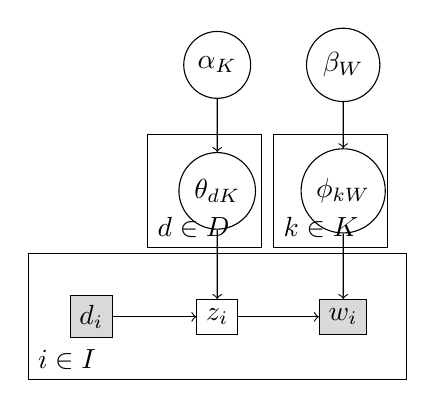
\begin{tikzpicture}[scale=.8]
\node (d) at (0,0) [BNVarDiscrete,BNObserved] {$d_i$};
\node (z) at (2,0) [BNVarDiscrete] {$z_i$};
\node (w) at (4,0) [BNVarDiscrete,BNObserved] {$w_i$};
\node (theta) at (2,2) [BNVar] {$\vmDK_{dK}$};
\node (phi) at (4,2) [BNVar] {$\vmKW_{kW}$};
\node (alpha) at (2,4) [BNVar] {$\vmK_K$};
\node (beta) at (4,4) [BNVar] {$\vmW_W$};
\draw [->] (d) -- (z);
\draw [->] (z) -- (w);
\draw [->] (alpha) -- (theta);
\draw [->] (theta) -- (z);
\draw [->] (beta) -- (phi);
\draw [->] (phi) -- (w);
\draw (-1,-1) rectangle (5,1);
\draw (-1,-1) node[above right] {$i\in I$};
\draw (.9,1.1) rectangle (2.7,2.9);
\draw (.9,1.1) node[above right] {$d\in D$};
\draw (2.9,1.1) rectangle (4.7,2.9);
\draw (2.9,1.1) node[above right] {$k\in K$};
\end{tikzpicture}
\end{minipage} &
$
\begin{array}{l}
\begin{array}{l}
p(\vmK_K\vmW_W\vmDK_{DK}\vmKW_{KW}z_Iw_I|d_I) =\\
\hspace{1cm}p(\vmK_K)p(\vmW_W)\\
\hspace{1cm}\prod_{d\in D}p(\vmDK_{dK}|\vmK_K)\prod_{k\in K}p(\vmDK_{kW}|\vmW_W)\\
\hspace{1cm}\prod_{i\in I}p(z_i|d_i\vmDK_{DK})p(w_i|z_i\vmKW_{KW})
\end{array}
\vspace{.3cm}
\\
\begin{array}{rcl@{\hspace{.5cm}}rcl}
\vmK_K & \sim & \cpnt{p}{K} & \vmW_W & \sim & \cpnt{p}{W}
\end{array}
\\
\begin{array}{r@{\hspace{.5cm}}rcl}
\forall d\in D & \vmDK_{dK}|\vmK_K & \sim & \mathbf{Dirichlet}(\vmK_K)\\
\forall k\in K & \vmKW_{kW}|\vmW_W & \sim & \mathbf{Dirichlet}(\vmW_W)\\
\forall i\in I & z_i|d_i\vmDK_{DK} & \sim & \mathbf{Cat}(\vmDK_{d_iK})\\
\forall i\in I & w_i|z_i\vmKW_{KW} & \sim & \mathbf{Cat}(\vmKW_{z_iW})
\end{array}
\end{array}
$
\end{tabular}
\begin{eqnarray}
\label{eqn:logprobtrue}
\log p(\vmK_K\vmW_W\vmDK_{DK}\vmKW_{KW}z_I|w_Id_I) & = &
\log\cpnt{p}{K}(\vmK_K)+\log\cpnt{p}{W}(\vmW_W)-D\log\mathcal{B}(\vmK_K)-K\log\mathcal{B}(\vmW_W)\\
\nonumber & + & \sum_{dk}(\vmK_k{-}1)\log\vmDK_{dk}+\sum_{kw}(\vmW_w{-}1)\log\vmKW_{kw}+\sum_{ik}\carac{z_i=k}(\log\vmDK_{d_ik}{+}\log\vmKW_{kw_i})
\end{eqnarray}
\caption{\label{fig:fullbn}The full Bayesian network of the LDA model and the decomposition of its joint distribution $q$.}
\end{figure*}
Given a number $D$ of documents, $W$ of words (or terms), $K$ of topics and $I$ of occurrences, a realisation consists of the following random variables\footnote{In the sequel, we take the convention of not distinguishing the vectors by typesetting them in boldface, but rather by systematically recalling their index ranges as subscripts.}: $(i)$ a tuple $(d_i,z_i,w_i)_{i\in I}$, where for each $i\in I$, the discrete objects $d_i\in D,z_i\in K,w_i\in W$ denote, respectively, the document, the topic and the word associated with occurrence $i$; $(ii)$ two stochastic matrices $\vmDK_{DK}$ (of dimension $D\times K$) and $\vmKW_{KW}$ (of dimension $K\times W$) which characterise each document $d$ as the distribution of topics $\vmDK_{dK}$ and each topic $k$ as the distribution of words $\vmKW_{kW}$; $(iii)$ two positive vectors $\vmK_K$ and $\vmW_W$ which characterise the topics and words of the whole collection. The full graphical representation of the LDA model is given in Figure~\ref{fig:fullbn}.

The space of realisations is that of complete collections of documents: this explains why the collection-level variables $\vmK_K$ and $\vmW_W$ are random, and not parameters. Besides the known size parameters $D,W,K,I$, the model has two possibly unknown parameters $\cpnt{p}{K}$ and $\cpnt{p}{W}$, which are distributions for $\vmK_K$ and $\vmW_W$, respectively. For the sake of symmetry, the occurrence-document vector $d_I$ is considered a random variable, but it is assumed always observed and independent of all the rest, so it could as well have been treated as a known parameter. All probability expressions are conditioned upon it. Conditioned to the observation of the occurrence-word vector $w_I$, the log probability is given, up to some additive constant depending only on $d_I,w_I$, by~(\ref{eqn:logprobtrue}).

Note that, at this point, we make no assumption on the distributions $\cpnt{p}{K}$ and $\cpnt{p}{W}$. Our main contribution is precisely in studying the impact of the choice of these distributions. We show that an appropriate choice leads to a new formulation of the variational approximation of LDA, which we investigate.
\section{PRIORS FOR VARIATIONAL BAYES LDA}
\label{sec:ldawithcprior}
The posterior probability given by~(\ref{eqn:logprobtrue}) does not admit an analytical expression. The VB method tries to approximate it, by projecting it onto a simpler space $\mathcal{C}$ of probability distributions, namely that of distributions $q$ of the form
\begin{equation}
\label{eqn:probvar}
\begin{array}{l}
q(\vmK_K\vmW_W\vmDK_{DK}\vmKW_{KW}z_I) = \cpnt{q}{K}(\vmK_K)\cpnt{q}{W}(\vmW_W)\\
\;\;\;\prod_{d\in D}q_d(\vmDK_{dK})\prod_{k\in K}q_k(\vmKW_{kW})
\prod_{i\in I}q_i(z_i)
\end{array}
\end{equation}
Hence, in the variational model, the variables $\vmK_K,\vmW_W,\{\vmDK_{dK}\}_{d\in D},\{\vmKW_{kW}\}_{k\in K},\{z_i\}_{i\in I}$ are assumed independent.
%%%%%%%%%%%%%%%%%%%%%%%%%%%%%%%%%%%%%%%%%%%%%%%%%%%%%%%%%%%%%%%%%%%%%%%%%%%
\subsection{The VB method}
%%%%%%%%%%%%%%%%%%%%%%%%%%%%%%%%%%%%%%%%%%%%%%%%%%%%%%%%%%%%%%%%%%%%%%%%%%%
The VB method solves the following optimisation problem:
\begin{eqnarray}
\label{eqn:KLmin}
q^* & = & \arg\min_{q\in\mathcal{C}}\divergence(q,\tilde{p})
\hspace{.3cm}\textrm{where}\hspace{.3cm}\tilde{p}=p|w_Id_I
\end{eqnarray}
Hence $q^*$ is the distribution of class $\mathcal{C}$, i.e. decomposable according to~(\ref{eqn:probvar}), which is closest, for the KL-divergence, to the posterior distribution $\tilde{p}$ given by~(\ref{eqn:logprobtrue}). VB computes an estimate $\dot{q}$ of $q^*$ in $\mathcal{C}$. It proceeds by simple coordinate descent, along the components $\dot{q}_X$, one for each independent variable $X$ in~(\ref{eqn:probvar}). The update, at each step of the coordinate descent focussing on variable $X$, is given by
\begin{eqnarray}
\label{eqn:vbcore}
\dot{q}_X(x) &\assignn\propto& \exp\expectation_{y\sim \dot{q}_{\neg X}}[\log\tilde{p}(x,y)]
\end{eqnarray}
where the expectation is taken over the set $\neg X$ of all the independent variables in~(\ref{eqn:probvar}) other than $X$. Hence, the estimate $\dot{q}$ converges to $q^*$, or at least to a local minimum of $\divergence(q,\tilde{p})$, taken to be an approximation of $\tilde{p}$. When the right-hand side in~(\ref{eqn:vbcore}) does not have an analytical expression, VB uses an additional approximation, by {\em externally} constraining the estimate $\dot{q}_X$ to be in a specific class of distributions. Typically, one may want to constrain $\dot{q}_X$ to be a Dirac distribution with some parameter $\dot{\pi}_X$ and the update becomes
\begin{eqnarray}
\label{eqn:vbcore-Dirac}
\dot{\pi}_X &\assignn& \arg\max_x\expectation_{y\sim \dot{q}_{\neg X}}[\log\tilde{p}(x,y)]
\end{eqnarray}
The right-hand side of~(\ref{eqn:vbcore-Dirac}) is the mode of the right-hand side distribution in~(\ref{eqn:vbcore}), since the closest Dirac approximation of any distribution is the Dirac at its mode.

In the case of the LDA model, it is well known that the choice of conjugate (Dirichlet) priors for variables $\vmDK_{DK}$ and $\vmKW_{KW}$ lead to update rules~(\ref{eqn:vbcore}) which {\em naturally} constrain the variational distributions to the following forms\footnote{To avoid a proliferation of Greek letters, we denote the variational parameters with the same letter as the corresponding model variables, decorated with a dot.}:
\[
\begin{array}{l@{\hspace{.3cm}}l}
\forall d\in D& \dot{q}_d(\vmDK_K) = \mathbf{Dirichlet}(\vmDK_K;\vvmDK_{dK}) \\
\forall k\in K& \dot{q}_k(\vmKW_W) = \mathbf{Dirichlet}(\vmKW_W;\vvmKW_{kW})
\end{array}
\]
Furthermore, $\dot{q}_i$ for $i\in I$ is by construction a categorical distribution, with some parameter $\vvmDWK_{iK}$. However, the resulting updates do not differentiate between the distributions $\dot{q}_i$ where $d_i,w_i$ are identical, i.e. multiple occurrences of the same word in the same document. Hence, the variational parameter $\vvmDWK_{IK}$ can be replaced by a parameter $\vvmDWK_{DWK}$ such that $\vvmDWK_{iK}=\vvmDWK_{d_iw_iK}$ for all $i\in I$. Likewise, the observation $d_I,w_I$ can be summarised by the sufficient statistics $n_{DW}$, which is the document-word count matrix:
\begin{eqnarray*}
n_{dw} & \triangleq & |\{i\in I|d_i=d,w_i=w\}|
\end{eqnarray*}
Finally, the updates given by~(\ref{eqn:vbcore}) applied to the LDA model are summarised in Figure~\ref{fig:ldaupdates}, where the different updates are given labels (in brackets under the arrow) for reference purpose. For clarity sake, we have introduced the intermediate variational quantities $\vvmbDK_{DK}$ and $\vvmbKW_{KW}$ defined by
\[
\vvmbDK_{dk}\triangleq\expectation_{\vmDK_K\sim\dot{q}_d}[-\log\vmDK_k]
\hspace{.3cm}
\vvmbKW_{kw}\triangleq\expectation_{\vmKW_W\sim\dot{q}_k}[-\log\vmKW_w]
\]
which have a simple analytical expression. One recognises in Figure~\ref{fig:ldaupdates} the standard updates of the LDA model, except maybe for the bottom two $\ruleref{d}$ and $\ruleref{w}$, discussed below.
\begin{figure*}
\[
\begin{array}{|rcl@{\hspace{1cm}}rcl|}
\hline
&&&&& \\[-.35cm]
\multicolumn{6}{|c|}{
\begin{array}{rcl}
\vvmDWK_{dwk} & \assign{K}\propto & \exp-(\vvmbDK_{dk}+\vvmbKW_{kw})
\end{array}
} \\
\vvmbDK_{dk} & \assignn & \Psi(\sum_{k'}\vvmDK_{dk'})-\Psi(\vvmDK_{dk}) &
\vvmbKW_{kw} & \assignn & \Psi(\sum_{w'}\vvmKW_{kw'})-\Psi(\vvmKW_{kw})\\
\vvmDK_{dk} & \assign{D} & \expectation[\cpnt{\dot{q}}{K}]_k+\sum_wn_{dw}\vvmDWK_{dwk} &
\vvmKW_{kw} & \assign{W} & \expectation[\cpnt{\dot{q}}{W}]_w+\sum_dn_{dw}\vvmDWK_{dwk} \\
&&&&& \\
\cpnt{\dot{q}}{K} & \assign{d}\propto & \cpnt{p}{K}\mbeta(-D,\sum_d\vvmbDK_{dK}) &
\cpnt{\dot{q}}{W} & \assign{w}\propto & \cpnt{p}{W}\mbeta(-K,\sum_k\vvmbKW_{kW})\\
\hline
\end{array}
\]
\caption{\label{fig:ldaupdates}Generic variational updates for the LDA model.}
\[
\begin{array}{|rcl@{\hspace{1cm}}rcl|}
\hline
&&&&& \\[-.35cm]
\vvmDK_{dk} & \assign{D} & \vvmK_k +\sum_wn_{dw}\vvmDWK_{dwk} &
\vvmKW_{kw} & \assign{W} & \vvmW_w^{-1}+\sum_dn_{dw}\vvmDWK_{dwk} \\
\vvmK_K & \assign{d} & \boldsymbol{\Phi}(\frac{1}{D}\sum_d\vvmbDK_{dK}) &
\vvmW_w & \assign{w} & \pmW_w+\sum_k\vvmbKW_{kw} \\
\hline
\end{array}
\]
\caption{\label{fig:ldaupdates-variant}Updates $\ruleref{D},\ruleref{W},\ruleref{d},\ruleref{w}$ in our variants: one is equivalent to the EM type 2 estimation method and the other is original. For the sake of presentation, we apply the former to the document-topic side and the latter to the topic-word side, but they are interchangeable, or the same variant could be applied to both sides.}
\end{figure*}
%%%%%%%%%%%%%%%%%%%%%%%%%%%%%%%%%%%%%%%%%%%%%%%%%%%%%%%%%%%%%%%%%%%%%%%%%%%
\subsection{Treatment of the parameters $\cpnt{p}{K}$ and $\cpnt{p}{W}$}
%%%%%%%%%%%%%%%%%%%%%%%%%%%%%%%%%%%%%%%%%%%%%%%%%%%%%%%%%%%%%%%%%%%%%%%%%%%
Let's first justify the update~$\ruleref{d}$ of $\cpnt{\dot{q}}{K}$ (the same applies to update~$\ruleref{w}$ of $\cpnt{\dot{q}}{W}$). By eliminating from~(\ref{eqn:logprobtrue}) all the terms which do not involve $\vmK_K$, hence contribute only a multiplicative constant, and taking expectations on the others, Equation~(\ref{eqn:vbcore}) becomes
\begin{small}
\begin{eqnarray*}
\cpnt{\dot{q}}{K}(\vmK_K)
& \assignn\propto &
\exp\log\cpnt{p}{K}(\vmK_K)-D\log\mathcal{B}(\vmK_K)\\
& + & \sum_d\expectation_{\vmDK_{dK}\sim\dot{q}_d}[\sum_k\vmK_k\log\vmDK_{dk}]\\
& = &
\cpnt{p}{K}(\vmK_K)\mathcal{B}(\vmK_K)^{-D}\exp\sum_{dk}-\vmK_k\vvmbDK_{dk}\\
& \propto &
\cpnt{p}{K}(\vmK_K)\mbeta(\vmK_K;-D,\sum_d\vvmbDK_{dK})
\end{eqnarray*}
\end{small}
where $\mbeta$ is the conjugate distribution of the Dirichlet in the exponential family introduced in Section~\ref{sec:huntingsnark}. Note that this formula, including the role of the $\mbeta$ distribution, holds in general, whatever the choice of priors $\cpnt{p}{K},\cpnt{p}{W}$. To make the updates of $\cpnt{\dot{q}}{K},\cpnt{\dot{q}}{W}$ concrete, we now need to proceed with that choice. Since the two variables $\vmK_K$ and $\vmW_W$ are parameters of Dirichlet distributions, on $\vmDK_{DK}$ and $\vmKW_{KW}$ respectively, we naturally choose their modelling distributions $\cpnt{p}{K},\cpnt{p}{W}$ in the conjugate class of Dirichlet, namely $\mbeta$. This {\em naturally} ensures that the corresponding variational distributions $\cpnt{\dot{q}}{K},\cpnt{\dot{q}}{W}$ are also in that class.

We first show that the so called EM type 2 hyper-parameter estimation, which has been proposed for VB LDA, is in fact a special case of this approach. Indeed, EM in general is known to be a special case of VB, and what we give here is just the pure VB presentation of the method, leading to the same updates. In VB, the method amounts to choosing an ``uninformative'' $\cpnt{p}{K}$, i.e. $\cpnt{p}{K}\propto1$, which is also the improper distribution $\mbeta(0,0)$. Reporting in~$\ruleref{d}$, this {\em naturally} constrains the distribution $\cpnt{\dot{q}}{K}$ to be equal to $\mbeta(-D,\sum_d\vvmbDK_{dK})$. However, update~$\ruleref{D}$ requires the computation of its expectation, which is intractable. Instead, $\cpnt{\dot{q}}{K}$ is {\em externally} constrained to be a Dirac distribution, hence we can apply Equation~(\ref{eqn:vbcore-Dirac}):
\[
\begin{array}{rcl}
\multicolumn{3}{c}{
\begin{array}{c@{\hspace{1cm}}c}
\cpnt{p}{K}\propto1 &
\cpnt{\dot{q}}{K} = \mathbf{Dirac}(\vvmK_K)
\end{array}
}\\
\vvmDK_{dk} & \assignn & \vvmK_k+\sum_wn_{dw}\vvmDWK_{dwk} \\
\vvmK_K & \assignn & \arg\max\mbeta(-D,\sum_d\vvmbDK_{dK})
\end{array}
\]
The $\arg\max$ expression above, computing the mode of the $\mbeta$ distribution, can be simplified by introducing function $\boldsymbol{\Phi}$ defined for any vector $u_N$ by
\begin{eqnarray*}
\boldsymbol{\Phi}(u_N) & \triangleq & \arg\min_{x_N}\log\mathcal{B}(x_N)+u_Nx_N
\end{eqnarray*}
The resulting update rules~$\ruleref{D}$ and ~$\ruleref{d}$ are given in Figure~\ref{fig:ldaupdates-variant}. By constraining $\cpnt{\dot{q}}{K}$ to be Dirac, the computation of its expectation becomes trivial in update~$\ruleref{D}$, but at the price of its own update~$\ruleref{d}$, which now requires the computation of the mode of the distribution thus approximated by the Dirac. In other words, we have traded a complex integration for a complex optimisation, but the latter is still more tractable than the former.

Let's now detail an alternative approach, which we call here ``full conjugacy'', on the topic-word side for the sake of presentation (but it works just as well on the document-topic side). We still choose $\cpnt{p}{W}$ in the $\mbeta$ class as before, but we don't force its parameter $(m,\pmW_W)$ to be $0$ as above. Hence, $\cpnt{\dot{q}}{W}$ is also in the same class, and let $(\dot{m},\vvmW_W)$ be its parameter. The updates are then straightforward to derive. The key observation here is that parameter $\dot{m}$ is assigned the expression $m-K$, which never changes in subsequent updates. Furthermore, if we choose $m=K$, that expression is null, i.e. $\dot{m}=0$. This is particularly helpful, because, then, the intractable $\mbeta(\dot{m},\vvmW_W)$ distribution becomes a simple Exponential distribution\footnote{We mean here a multivariate Exponential, product of independent scalar Exponentials.} with rate $\vvmW_W$, the expectation of which is trivial to compute.
\[
\begin{array}{rcl}
\multicolumn{3}{c}{
\cpnt{p}{W} = \mbeta(K,\pmW_W)
\;\;
\cpnt{\dot{q}}{W} = \textbf{Expon}(\vvmW_W)
} \\
\vvmKW_{kw} & \assignn & \vvmW_w^{-1}+\sum_dn_{dw}\vvmDWK_{dwk} \\
\vvmW_w & \assignn & \pmW_w+\sum_k\vvmbKW_{kw}
\end{array}
\]
The resulting update rules~$\ruleref{W}$ and  $\ruleref{w}$ are given in Figure~\ref{fig:ldaupdates-variant}. Note that parameter $\pmW_W$ is still free: it could be set to $0$, or preferably to some small machine value (the same for all components) to avoid numerical instability in the inversion of the rate defining the expectation of the Exponential in rule~$\ruleref{W}$.
%%%%%%%%%%%%%%%%%%%%%%%%%%%%%%%%%%%%%%%%%%%%%%%%%%%%%%%%%%%%%%%%%%%%%%%%%%%
\subsection{Discussion}
%%%%%%%%%%%%%%%%%%%%%%%%%%%%%%%%%%%%%%%%%%%%%%%%%%%%%%%%%%%%%%%%%%%%%%%%%%%
In both variants of LDA, the priors are improper: in the EM type 2 estimation, because it is ``uniform'' on a space of infinite measure (the positive orthant), and in the full conjugacy method, by Proposition~\ref{prop:mbeta-proper}, since $K$ is obviously not less than $1$.

Using an improper prior is not a problem so long as the posterior is guaranteed to remain proper. While we cannot check that on the true posterior, we can at least check that its approximation computed by the VB method is proper. For the full conjugacy method, $\cpnt{\dot{q}}{W}$ is an Exponential, and obviously proper: it is easy to show that its parameter $\cpnt{\vvmW}{W}$ always remain strictly within the positive orthant. As for the EM type 2 method, $\cpnt{\dot{q}}{K}$ is a Dirac, but we should rather consider the distribution which it approximates, namely $\mbeta(-D,\sum_d\vvmbDK_{dK})$, and show that the latter is proper. By Proposition~\ref{prop:mbeta-proper}, and after a few transformations (essentially replacing $\vvmbDK_{DK}$ by its definition in terms of $\vvmDK_{DK}$) we have to show
\[
\log\sum_k\exp\frac{1}{D}\sum_d\Psi(\vvmDK_{dk})<\frac{1}{D}\sum_{d}\Psi(\sum_k\vvmDK_{dk})
\]
And indeed, this is a direct consequence of the convexity of $\log\sum\exp$, together with some known property of function $\Psi$.

The prior of the full conjugacy method is very different in shape from that of the EM type 2 method. While the latter has a uniform (improper) density, the former is strongly peaked at $0$ and sharply decreasing away from it. It tends to favour values of $\vmW_W$ close to $0$. But $\vmW_W$ is the parameter of the Dirichlet for $\vmKW_{kW}$, and a Dirichlet with parameter close to 0 tends to favour values towards the borders, and even more the corners, of the simplex. This is indeed confirmed by looking at the shape of the (improper) prior distribution of the whole matrix $\vmKW_{KW}$, which can be computed analytically by collapsing $\vmW_W$. Since $\vmKW_{kW}$ is the distribution of words of topic $k$, being close to the borders and corners of the simplex essentially means being sparse. Hence, our choice of prior favours sparsity in the topic word profiles (the same applies to the document topic profiles if we apply full conjugacy on that side).

The document topic side and the topic word side of the LDA model are strictly symmetric, just as dimensions are treated symmetrically in a matrix factorisation. However, when considering the asymptotic behaviour of the model, that symmetry is broken, as the vocabulary is often seen as fixed, while the number of documents can grow to infinity. In that case, our full conjugacy variant could not be applied to the document topic side of the model, since it would make its prior $\cpnt{p}{K}=\mbeta(D,\pmK_K)$ dependent on the size $D$ of the document collection, and it would not asymptotically vanish as is usually expected. On the other hand, the topic word side is not affected, as the corresponding prior depends only on the number of topics $K$.
\section{EXPERIMENTS}
\section{DISCUSSION}

\subsubsection*{References}

\end{document}
